A Figura ~\ref{fig:cadeiraOctomap} apresenta um exemplo dos resultados obtidos com o uso do pacote \verb|octomap|. Em ~\ref{fig:cadeiraOctomap}(b) é mostrada a cena capturada pela câmera convencional do Kinect e, em ~\ref{fig:cadeiraOctomap}(a) a saída do OctoMap. É possível verificar a precisão deste método sabendo que cada quadrado tem resolução de $5cm$, escolhido no \textit{launcher} do OctoMap, e a cadeira tem $40cm$ de largura. Após a contagem dos quadrados, podemos concluir que o modelo gerado está muito próximo do real pois o encosto tem 9 quadrados de largura.

\begin{figure}[H]
\centering
\begin{tabular}{cc}
  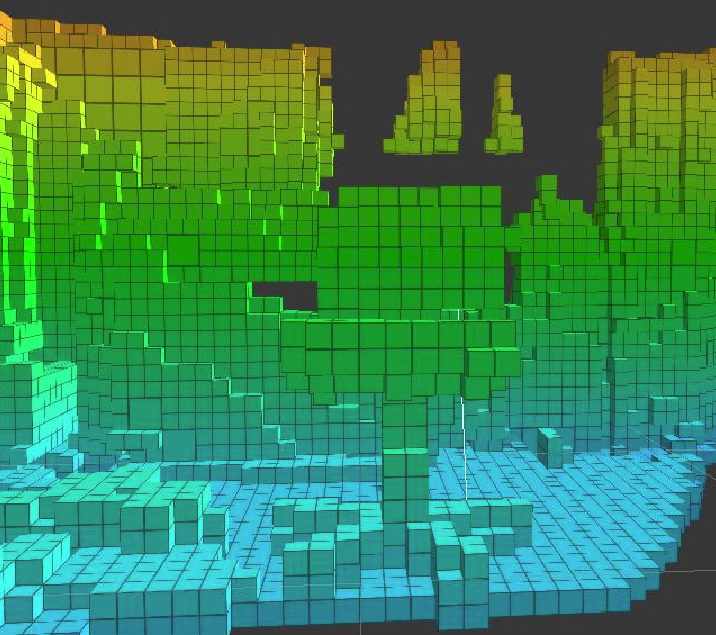
\includegraphics[width=6cm, height=6cm]{images/cadeiraOctomap.PNG} &
  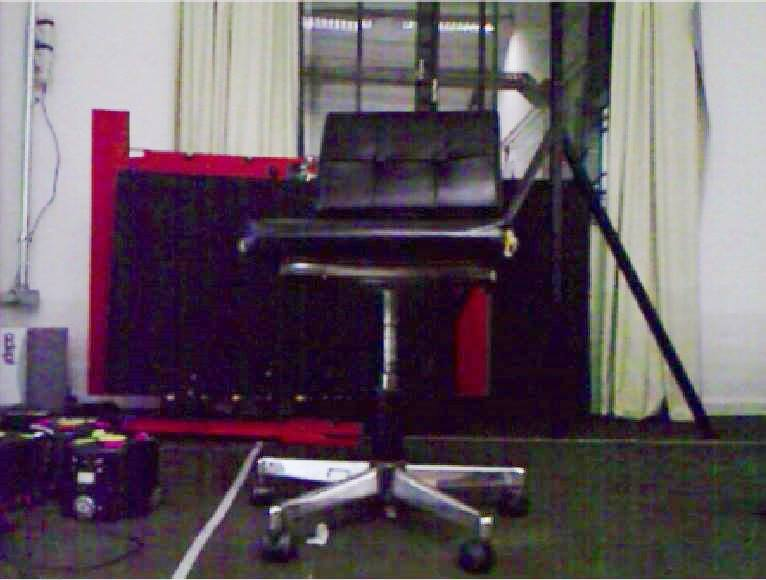
\includegraphics[width=6cm, height=6cm]{images/cadeiraKinect.jpg} \\
 (a) & (b)
\end{tabular} 
\caption{\small{(a) Resultado obtido com OctoMap \cite{hornung13auro}. (b) Imagem capturada da câmera do Kinect.}}
\label{fig:cadeiraOctomap}
\end{figure}

Foram feitos testes com o pacote e ele se mostrou eficiente computacionalmente, sendo possível mapear ambientes internos de diferentes tamanhos sem grandes problemas, mesmo no \textit{netbook}, que é o \textit{master} do ROS. Quanto aos problemas, foram encontrados alguns erros percetíveis ao fazer o mapeamento dos ambientes de teste:

\begin{compactitem}
\item Muitas vezes, ao fazer o mapeamento de algum local o pacote  marca um mesmo objeto duas vezes em posições ligeiramente diferentes, poluindo a visualização e não representando fielmente a realidade. Esse problema se repete até mesmo em ambientes simulados e trata-se de um problema conhecido do pacote. Neste momento, uma melhoria neste comportamento encontra-se fora do escopo do projeto.
\item Nos primeiros testes o sistema de coordenadas de referência considerado era o \verb|odom| (responsável pela odometria), sendo que os erros cumulativos de odometria causavam erros, algumas vezes, consideráveis. Para fim de testes, foi usado o sistema de localização \verb|gmapping| (em parte responsável pelo SLAM) e adotado o sistema de coordenadas de referência \textit{map} (criado pelo \verb|gmapping|), o que não trouxe melhoras significativas.
\end{compactitem}